% ******************************* Thesis Appendix B ********************************

\chapter{Description of application examples}

\ifpdf
    \graphicspath{{Appendix2/Figs/Raster/}{Appendix2/Figs/PDF/}{Appendix2/Figs/}}
\else
    \graphicspath{{Appendix2/Figs/Vector/}{Appendix2/Figs/}}
\fi

%******************************************************************************************
%******************************************************************************************
\section{Nuclear power plant in Paks, turbine hall}
\label{sec:paks}

%******************************************************************************************
\subsection{Overview}

The Paks Nuclear Power Plant is the only nuclear power plant in Hungary and it covers about $50 \%$ of the Hungarian electricity demand. The plant was commissioned in 1982 and its operational time was recently extended by 20 years up to the thirties. Due to its importance and severe consequences of potential failures, regular probabilistic risk assessment is required and performed on the facility. The candidate participated in a comprehensive probabilistic assessment of the facility's load bearing structures and in the development of an improved methodology for fragility curve based probabilistic assessment. From this project the turbine hall is selected to demonstrate the findings of this study. It is a regular steel hall housing the turbines that convert thermal energy into kinetic one. The reliability of the hall is crucial for the reliable performance of the whole facility.

%******************************************************************************************
\subsection{Fragility curves}

The reliability of the hall is governed by the system like failure of multiple frames. Furthermore, multiple truss members and failure modes contribute to the failure probability of each frame. For simplicity only a single frame with its governing failure mode is considered. This characterizes well the whole hall system and deemed sufficient for illustration. The location of the selected frame is shown in Figure~\ref{fig:main_building_overview}. The main dimensions with the governing limit states are illustrated in Figure~\ref{fig:frame_fragi}. The corresponding component and system (series) level fragility curves\footnote{Fragility curve is a cumulative distribution function with each ordinate is expressing a conditional probability.} are also presented. In this thesis the $g_2$ limit state function is used in all analyses of the turbine hall.

\begin{figure}[htbp!] 
	\centering    
	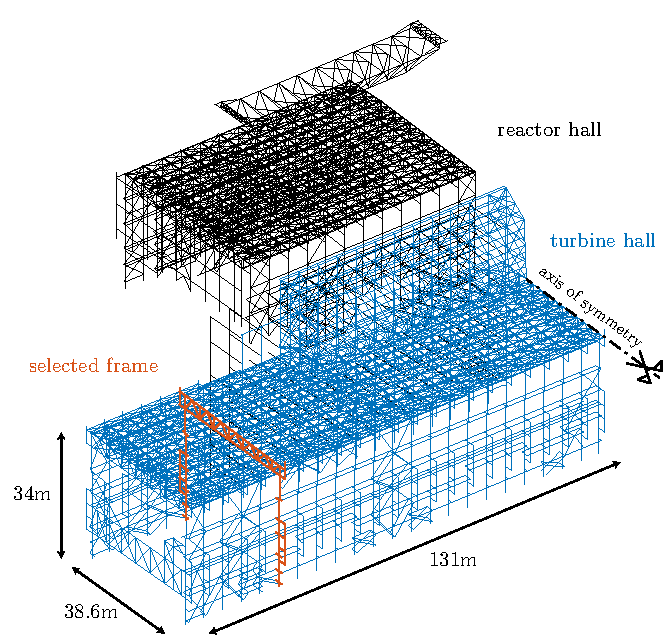
\includegraphics[]{main_building_overview_02.pdf}
	\caption{Main building of Paks Nuclear Power Plant with the selected frame (orange).}
	\label{fig:main_building_overview}
\end{figure}


\begin{figure}[htbp!] 
	\centering    
	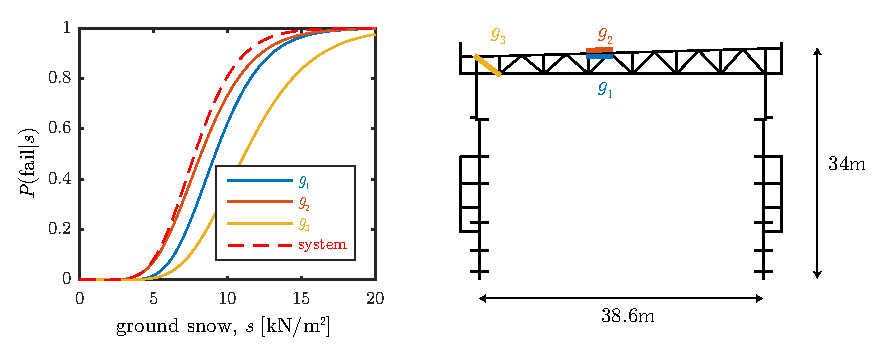
\includegraphics[]{frame_28(26)_fragility.pdf}
	\caption{Selected frame of turbine hall (right) and its fragility curves (left) for governing failure modes. In this thesis the $g_2$ limit state function (orange) is used in all analysis of the turbine hall.}
	\label{fig:frame_fragi}
\end{figure}

For our current purpose it is sufficient to know the fragility curves; further details on how these were obtained can be found in \citet{PaksMethod2014, PaksAppl2014}.

%******************************************************************************************
\subsection{Snow action}
The probabilistic model of ground snow load is inferred from the snow water equivalent data of CarpatClim database \citep{Szalai2013}. The gridpoint with latitude 46.6°N and longitude 18.9°E geographical coordinates is used to obtain the ground snow load for the power plant. The observations are available for 49 full winter seasons (Figure~\ref{fig:amax_year_paks}). The main statistics of the annual (winter season) maxima are given in Table~\ref{tab:paks_snow}.

Reference period of one year is used in all calculations related to the turbine hall. This follows the common practice in probabilistic risk assessment of nuclear power plants.

\begin{figure}[htbp!] 
	\centering    
	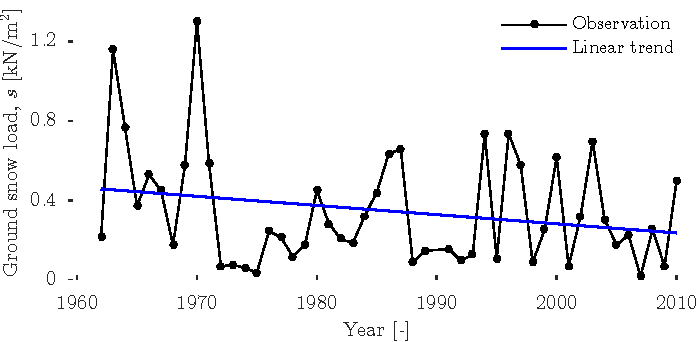
\includegraphics[]{amax_year_paks.pdf}
	\caption{Annual ground snow maxima and linear trend for Paks Nuclear Power Plant site.}
	\label{fig:amax_year_paks}
\end{figure}

\begin{table}
\caption{Main statistics of annual ground snow maxima for Paks Nuclear Power Plant site.}
\centering
\label{tab:paks_snow}
\small
	\begin{threeparttable}
    \begin{tabular}{m{0.45\textwidth}  m{0.2\textwidth}}
    \toprule
    Statistics  & Value \\
    \midrule
    \rowcolor{lightgrey} Sample size & 49 \\
    Mean & 0.35 kN/m$^2$ \\
    \rowcolor{lightgrey} Coefficient of variation (bias corrected) & 0.83 \\
    Skewness (bias corrected) & 1.34 \\
    \rowcolor{lightgrey} Characteristic value\tnote{*} & 1.10 kN/m$^2$ \\
    GEV shape coefficient ($\xi$)\tnote{\textdagger} & 0.40 \\
    \bottomrule
    \end{tabular}
    \begin{tablenotes}
    	\item[*] 0.98 fractile of Gumbel distribution fitted with method of moments in line with \citet{Sanpaolesi1998}.
	    \item[\textdagger] Obtained using maximum likelihood method and belongs to Fréchet familiy.  
   	\end{tablenotes}
   	\end{threeparttable}
\end{table}


%******************************************************************************************
%******************************************************************************************
\section{Locomotive workshop in Budapest, Eiffel-hall}
\label{sec:eiffel}

\subsection{Overview}
The Eiffel-hall of Budapest is a more than 130 years old wrought iron structure that is up to recently served as one of the largest locomotive workshop in Hungary. The workshop has closed its doors in 2009 and afterwards the structure was classified as a historical monument. Soon it was designated to a government flagship project with the intention to serve the Hungarian State Opera House and the Erkel Theatre as a workshop and rehearsal center, while preserving the original structures and architectural style.

It is a 95~m $\times$ 235~m $\approx$ 22000~m$^2$ floor area hall that is presumably erected between 1883 and 1885. The riveted truss structure has five adjacent halls and made of wrought iron. Semi-probabilistic calculations revealed that snow is the governing action for many structural elements and substantial portion of the roof should be heated to avoid hazardous snow accumulation. Probabilistic analysis of the structure was to be undertaken due to (\textit{i}) the importance and value of the structure; (\textit{ii}) the inadequacy of current standardized methods to handle existing structures, e.g. to account for survived years.

\subsection{Selected truss member and failure mode}

Strength ultimate limit state of a purlin is selected as representative failure mode. The purlin is located in a side hall (Figure~\ref{fig:eiffel_hall_overview}) and its failure mode corresponds to the plastic rupture of a truss member under tension (Figure~\ref{fig:selected_purlin}). For simplicity solely this failure mode is considered albeit the failure probability of structure is governed by system like behavior. The reliability of the purlin is analyzed considering the conditions expected to be present after the refurbishment and neglecting the earlier survived years. The details of the involved random variables and formulation of the limit state function can be found in \cite{Eiffel2016}. 

\begin{figure}[htbp!] 
	\centering    
	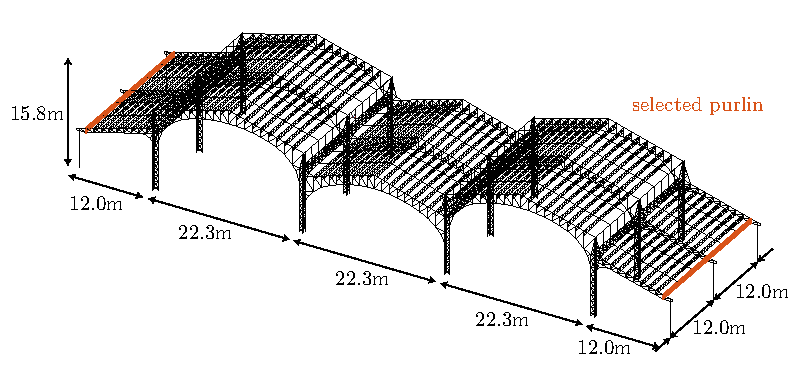
\includegraphics[]{eiffel_hall_overview2_db.pdf}
	\caption{Overview of the Eiffel-hall with the selected truss purlin (orange).}
	\label{fig:eiffel_hall_overview}
\end{figure}

\begin{figure}[htbp!] 
	\centering    
	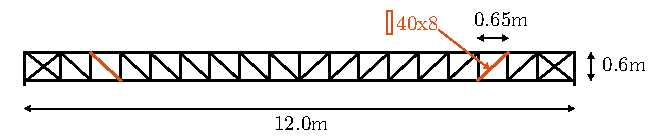
\includegraphics[]{selected_purlin.pdf}
	\caption{Selected truss purlin with governing truss member (orange). In this thesis this highlighted member is used in all analysis of the Eiffel-hall.}
	\label{fig:selected_purlin}
\end{figure}

\subsection{Snow action}
The snow water equivalents are obtained from the CarpatClim database \citep{Szalai2013}. The gridpoint with latitude 47.5°N and longitude 19.1°E geographical coordinates is used to obtain the ground snow load for the site. The observations are available for 49 full winter seasons (Figure~\ref{fig:amax_year_eiffel}). The main statistics of the annual (winter season) maxima are given in Table~\ref{tab:eiffel_snow}.

Reference period of 50 years is used in all calculations related to the Eiffel-hall. This is in line with the practice of reliability assessment of common engineering structures.

\begin{figure}[htbp!] 
	\centering    
	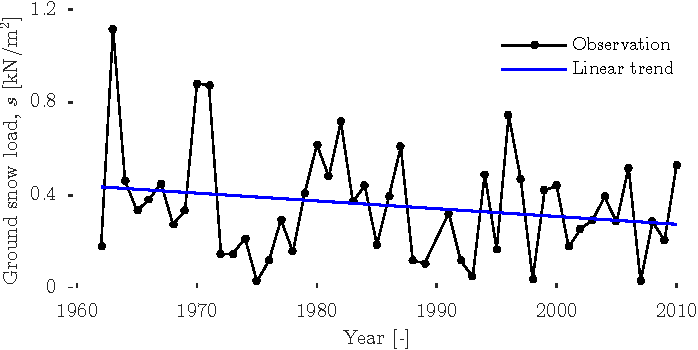
\includegraphics[]{amax_year_eiffel.pdf}
	\caption{Annual ground snow maxima and linear trend for Eiffel-hall site.}
	\label{fig:amax_year_eiffel}
\end{figure}

\begin{table}
\caption{Main statistics of annual ground snow maxima for Eiffel-hall site.}
\centering
\label{tab:eiffel_snow}
\small
	\begin{threeparttable}
    \begin{tabular}{m{0.45\textwidth}  m{0.2\textwidth}}
    \toprule
    Statistics  & Value \\
    \midrule
    \rowcolor{lightgrey} Sample size & 49 \\
    Mean & 0.36 kN/m$^2$ \\
    \rowcolor{lightgrey} Coefficient of variation (bias corrected) & 0.67 \\
    Skewness (bias corrected) & 1.06 \\
    \rowcolor{lightgrey} Characteristic value\tnote{*} & 0.97 kN/m$^2$ \\
    GEV shape coefficient ($\xi$)\tnote{\textdagger} & 0.05 \\
    \bottomrule
    \end{tabular}
    \begin{tablenotes}
    	\item[*] 0.98 fractile of Gumbel distribution fitted with method of moments in line with \citet{Sanpaolesi1998}.
	    \item[\textdagger] Obtained using maximum likelihood method and belongs to Fréchet familiy.  
   	\end{tablenotes}
   	\end{threeparttable}
\end{table}


